\documentclass{my}
%\documentclass{article}
\usepackage{url}


\ifx\pdfoutput\undefined
% we are running LaTeX, not pdflatex
\usepackage{graphicx}
\else
% we are running pdflatex, so convert .eps files to .pdf
%\usepackage[pdftex]{graphicx}
%\usepackage{epstopdf}
\fi 

\copyrightyear{}
\pubyear{}

\newcommand{\pr}[1]{\mbox{\sf #1}}
\def\OMIM{\pr{OMIM}}
\def\OrdoGroup{\pr{OrdoGroupOfDiseases}}


% Equation
\newcommand{\eqnref}[1]{Equation~\ref{eqn:#1}}
\newcommand{\eqnlabel}[1]{\label{eqn:#1}}

\newcommand{\tbleqn}[1]{
\begin{math}
\begin{aligned}[1]
#1
\end{aligned}
\end{math}
}

\begin{document}
\firstpage{1}

\title{k-BOOM: A Bayesian approach to ontology structure inference, with applications in disease ontology construction}

\author{Christopher J. Mungall\,$^{1}$\footnote{to whom correspondence should be addressed},
  Sebastian Koehler\,$^{2}$
  Peter Robinson\,$^{2}$
  Ian Holmes\,$^{3}$
  Melissa Haendel\,$^{4}$
}
\address{
  $^{1}$Environmental Genomics and Systems Biology Division, Lawrence Berkeley National Laboratory, MS977, 1 Cyclotron Road, Berkeley, CA 94720 USA\\
  $^{2}$Institute for Medical and Human Genetics, Charit\'{e}-Universit\"atsmedizin Berlin, Augustenburger Platz 1, 13353 Berlin, Germany. \\
  $^{3}$Department of Bioengineering, University of California, Berkeley, CA, USA \\
  $^{4}$Department of Medical Informatics \& Clinical Epidemiology, Oregon Health and Sciences University, Portland, Oregon, USA
}

\history{}

\editor{}

\maketitle

\section{Abstract}

One strategy for building ontologies covering domains such as disease
or anatomy is to weave together existing knowledge sources (databases,
vocabularies and ontologies) into single cohesive whole. A first step
in this process is to generate \emph{mappings} between the elements of
these different sources. There are a number of well-known techniques
for generating mappings, both manual and automatic. Sometimes mappings
are seen as an end in themselves, with the sources remaining in a
loosely connected state. However, if we want to take the next step and
use the mappings to weave together the different sources into a
cohesive reference ontology, then we need to translate the mappings
into precise logical relationships. This will allow us to safely merge
equivalent concepts, creating a unified ontology. This translation is
a non-trivial step, as each mapping can be interpreted as multiple
different logical relationships, with each interpretation affecting
the likelihood of the others. There is a lack of automated methods to
assist with this last step; this resolution is typically performed by
expert ontologists.

Here we describe an ontology construction technique that takes
two or more ontologies linked by hypothetical axioms, and estimates
the most likely unified logical ontology. Hypothetical axioms can
themselves be derived from semantically loose mappings. The method
combines deductive reasoning and probabilistic inference and is called
Bayesian OWL Ontology Merging (BOOM). We describe a special form
k-BOOM that works by factorizing the probabilistic ontology into $k$
submodules. We also briefly describe a supplemental lexical and
knowledge-based technique for generating a set of hypothetical axioms
from loose mappings.

We are currently using this technique to build a merged disease
ontology (Monarch Disease Ontology; MonDO) that unifies a broad range
of vocabularies into a consistent and coherent whole.


\section{Introduction}

Ontologies provide a cohesive representation of some knowledge domain,
such as human anatomy or human disorders. One of the
characteristic features of an ontology is that relationships between
elements have precise logical interpretations, usually expressed in the Web
Ontology Language (OWL). For some domains, such as cellular biology,
we have consensus reference ontologies such as the Gene Ontology, with
broad and deep coverage of the domain. In other areas, such as
diseases) there are multiple ontologies and databases with distinct
perspectives and overlapping content. Here no single ontology provides
the complete picture, so we would like to weave these together into a
unified cohesive whole. The most common approach here is to generate
mappings connecting classes or database entities. However, mappings
are only one step towards producing a unified ontology. Most mappings
lack clear semantics, and so cannot be used effectively for reasoning
in a description logic environment. Additionally, mappings are
typically not enough to merge classes from two ontologies into a
common class, unless we are guaranteed the mapping represents true
equivalence. This is illustrated in figure \ref{fig:mapping-example},
which shows mappings between classes in three vocabulary
sources.

%----------------------------------------
\begin{figure}
\center
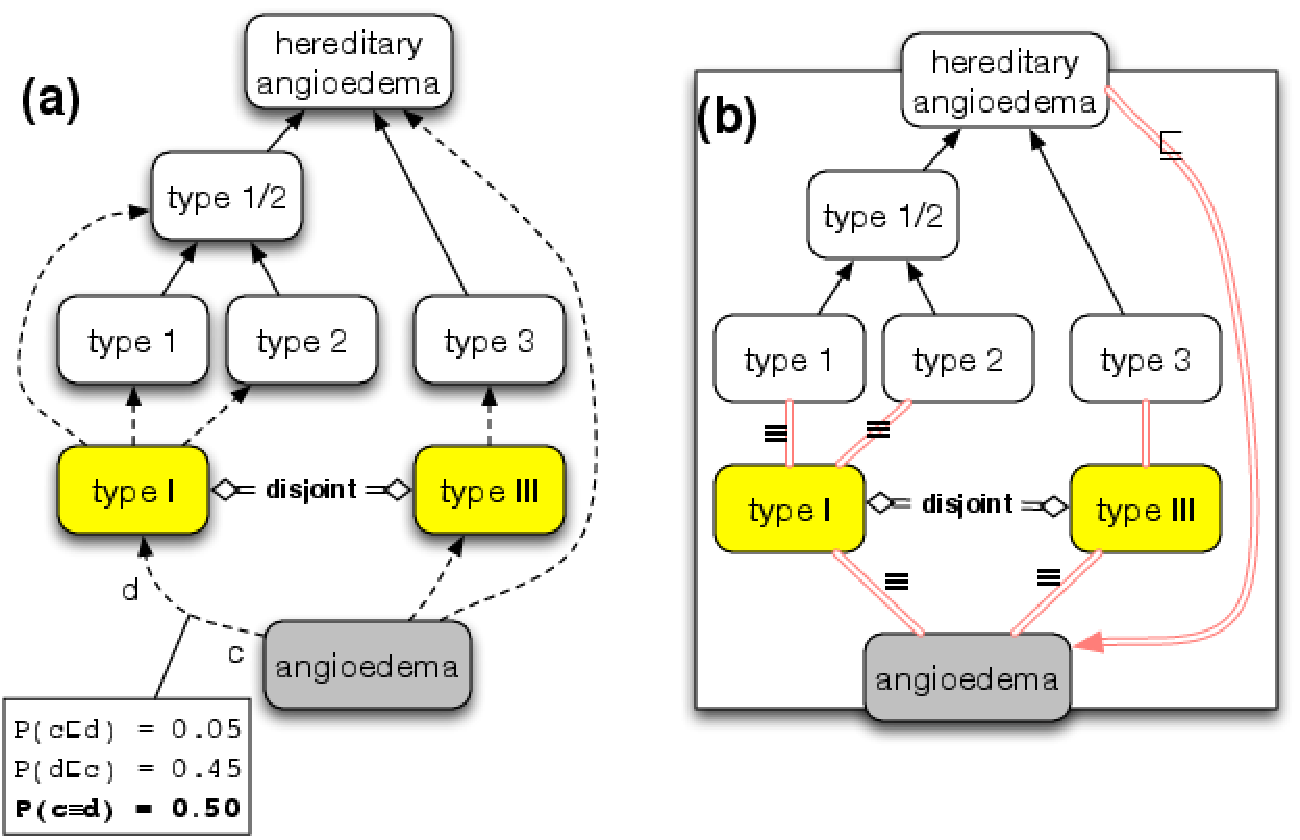
\includegraphics[width=7.5cm]{mapping-example}
\caption{(a) Mappings between 3 vocabularies (shown in different
  colors). Logical relationships (axioms) within an ontology
  (subsumption) shown in solid lines, Arrows denote SubClassOf
  (e.g. \emph{type-1} $\sqsubseteq$ \emph{type-1/2}). In the yellow
  ontology, types 1 and 3 are declared \emph{Disjoint} (i.e. no shared
  subclasses). Dashed lines represent loose mappings (b) one possible
  configuration with hypothetical axioms derived from mappings shown
  as double red lines. In this example, all mappings interpreted as
  equivalence ($\equiv$) except \emph{hereditary angioedema}
  $\sqsubseteq$ \emph{angioedema} (white to grey). Note that due to
  the logical properties of $\sqsubseteq$ and $\equiv$ all nodes in
  the enclosing box are inferred to be in a mutually equivalent
  clique, yielding incoherency (via disjointness axiom).}
\label{fig:mapping-example}
\end{figure}
%----------------------------------------

We have devised and implemented an algorithm called kBOOM that assists
a biocurator in merging ontologies. The kBOOM algorithm takes as input
a \emph{probabilistic} ontology which consists of a combination of
logical axioms and hypothetical axioms, and returns the most likely
ground ontology. Hypothetical axioms can be generated using a variety
of methods, including using pre-defined curated mappings. The
resulting ontology will include only precise logical axioms
connecting classes, such as SubClass ($\sqsubseteq$) and Equivalence
($\equiv$) axioms. Any classes connected via equivalence axioms can be
safely merged (i.e. merging produces a structure with the same logical entailments)

We are applying kBOOM to merge a mixture of ontologies, databases and
vocabularies which describe diseases or disorders, into the Monarch
Disease Ontology (MonDO), because no one single
source provides a comprehensive picture of the disease space. For
example, the Disease Ontology (DOID)\cite{Kibbe2014} provides a broad
classification of disease types, but does not enumerate all the
diseases in Online Mendelian Inheritance in Man
(OMIM)\cite{amberger2015}. Conversely, OMIM provides largely a flat
list without a hierarchy, and typically only covers disorders with genetic
etiology. Orphanet\cite{rath2012} has an emphasis on rare disease, and
employs different classification criteria from DOID. When previous
attempts have been made to unify these, the results are frequently
incomplete. For example, MedGen\cite{coordinators2015database} includes OMIM and Orphanet, but many
of the entries, such as that for \emph{Hyperekplexia hereditary} lack
a classification. Here we explore an ontology merging strategy as one possible solution to this problem.

\section{Methods}

Our approach takes a collection of ontologies $O_1,...,O_v$, and
produces a coherent well-connected merged ontology $O^M$, in which the
classes are connected using OWL logical axioms. We include
vocabularies and databases in our definition of ontology. The input
may also include a set of previously curated mappings $M \in C \times
C$, where $C$ is the total set of classes in all sources. We assume
that a mapping means that the two classes have some substantial degree
of similarity, but do not assume any logical semantics.

Our approach consists of a pipeline with two steps:

\begin{enumerate}
\item \emph{Generation of a probabilistic ontology with prior probabilities}. Prior probabilities can be generated using a variety of methods, such as lexical approaches, or by using existing curated mappings.
\item \emph{Estimation of the most likely ontology}. We attempt to maximize the posterior probability for different combinations of axioms, utilizing the complete OWL semantics\footnote{https://www.w3.org/TR/owl2-direct-semantics/}. Once this has been determined, additional post-processing can be performed, such as merging equivalent classes.
\end{enumerate}

We focus on this second step as it constitutes a novel method, and the
primary contribution of this paper. We first describe the
\emph{general} approach which is applicable to OWL ontologies of any
expressivity, and we then describe a \emph{specific} approach which
can be applied to simpler ontologies in which the probabilistic aspect
utilizes only concept inclusion and equivalence axioms.

To illustrate the first step with a concrete example, we give an
example of a procedure for estimating prior weights for disease
ontology mappings, and outline how we are using the combined procedure
to build the Monarch merged disease ontology (MonDO).

\subsection{Ontology structure inference: general approach}

\subsubsection{Probabilistic Ontologies}

The input to the structure inference procedure is a \emph{probabilistic ontology}:

\begin{equation}
O^P = \langle A,H \rangle
\end{equation}

where $A$ consists of \emph{logical axioms} $A_1,...,A_l$, and $H$ consists of \emph{hypothetical axioms}
$H_1,...,H_n$.

Both of these axiom sets involve any combination of
classes from the union of sources, which we denote $C$. However, a
common use case is that $A$ consists purely of within-source
axioms (e.g. two independent disease ontologies) and $H$ consists of
hypothetical axioms derived from cross-ontology mappings.

The joint probability distribution (JPD) is:

\begin{equation}
P(O^P) = P(H,A) = P(H)P(A|H)
\end{equation}
\begin{equation}
P(O^P) = \prod_{H_i \in H}P(H_i = h_i)P(A|H)
\eqnlabel{JointLikelihood}
\end{equation}

where $h_i$ is a boolean representing the truth value of hypothetical axiom $H_i$

For $P(A|H)$ we assume a uniform probability, except in the case
where the ontology $O^P$ is \emph{incoherent}, i.e. there exists a
class $c \in C$ such that $c$ is \emph{unsatisfiable}, where $unsat(c)
= O^P \vDash c \equiv \perp$. This situation can arise whenever the
ontology violates any logical constraints, encoded in OWL.  This state
can be checked using a standard deductive OWL reasoner.

We attempt to find the most likely ontology, i.e. set of values
$h_1,...,h_n$ that maximizes the posterior probability.

As there are $2^{|H|}$\ combinations, we use a number of techniques
to reduce the search space. For the first of these, we \emph{factorize}
the calculation by splitting the ontology into sub-modules.

\subsubsection{Factorization via module extraction}

A \emph{modularization} procedure takes an ontology $O$ and produces
ontology modules. We can apply the analogous procedure to
probabilistic ontologies and produce $k$ probabilistic modules. A
number of different modularization strategies can be applied. For some
problems it may be possible to produce $k$ modules that are
independent, in which case the probability can be factorized as:

\begin{equation}
P(O^P) = \prod_{k \in N}P(O^P_k)
\eqnlabel{Factorization}
\end{equation}

In other cases, modules may have dependencies; we do not cover this
here, approaches may involve Bayes networks or factor graphs.

\subsubsection{Greedy selection search procedure}

Even after factorization, the number of possibilities may still be
prohibitive (a module size of 100 nodes is not atypical, which has $4^100$ configurations).
In order to further reduce the search space, we apply a
greedy approach. Here, when searching for solutions for any module
$O_k$ we iteratively take the axiom for $H_k$ with the highest
probability and assume it to be true. We repeat this until the number
of hypothetical axioms is reduced to a user-specified threshold $T$.

We immediately reject any axioms that lead to $O^P$ becoming
incoherent. Additionally, we prospectively prune any axioms in $H_k$
that will themselves lead to incoherency, or that have become
logically entailed.

We attempt to re-modularize at each stem: the selection procedure may
lead to the current module being splittable into sub-modules.

Future extensions include the use of MCMC methods.

\subsection{Ontology structure inference: Approach for $AL^{-}$-ontologies}

We have implemented a procedure for inferring ontology structures
where the hypothetical axioms consist only of only the
$\sqsubseteq$\ (SubClass) or $\equiv$\ (Equivalence) constructs,
applied between two named classes $C_i, C_j \in C$. Formally:

\begin{equation}
H \subset \{  C_i \sqsubseteq C_j : i,j \in C \} \cup \{  C_i \equiv C_j : i,j \in C \}
\end{equation}

This is a subset of the Description Language AL (Attributive
Language), which we denote $AL^{-}$. Note we do not restrict the expressivity of
the non-hypothetical logical axioms $A$.

Limiting the expressivity of the probabilistic subset reduces the
search space, as there are fewer possibilities. For any pair of
classes $c,d$ in a mapping, there are only four possibilities: $c \sqsubset d$, $d \sqsubset c$, $c \equiv d$, $c \not\sqsubseteq d \wedge d \not\sqsubseteq c $. This
limitation also allows for the extraction of smaller modules.

For the ontology mapping use case, we also assume an additional
logical constraint in the form of \emph{AllDistiguishableFrom}
axioms. Here we assign each class in the ontology to a \emph{source},
and we constrain such that there are no equivalent pairs of classes
within a source.

\begin{equation}
C_i \in S, C_j \in S, C_i \neq C_j \to C_i \not\equiv C_j
\end{equation}

\subsubsection{Extracting Locally Independent Modules for $AL^{-}$}

By limiting the probabilistic subset to only SubClass and Equivalence
axioms, we can exhaustively partition the ontology into independent
submodules, based on whether the probability of any two members of the
partition being equivalent is non-zero.

Here we split the ontology into $k$ modules such that each module is
independent. We take all hypothetical equivalence axioms in $H$ and
assume $P(H_i=true)=1$, thus creating a \emph{maximally equivalent}
ontology $O'$ (see figure \ref{fig:mapping-example}b for example). We
then obtain the set of all entailed equivalence cliques $N$ from $O'$
(using any reasoner that is complete for the profile of $A$). For this
step, we ignore logical axioms such as disjointness axioms that can
lead to incoherency.

We then iterate through all cliques $N_1,...,N_n \in N$ and extract a
probabilistic module $O^{N_i}$, where the module contains all classes
in $N_i$, plus all logical axioms in $A$ that reference any class in
$N_i$, plus all hypothetical axioms in $H$ that connect a class in
$N_i$.

This corresponds to the factorization in \eqnref{Factorization}.


\subsubsection{Estimating prior edge probabilities for disease mappings}

kBOOM takes as inputs hypothetical axioms with assigned prior
probabilities. For this, we make use of existing mappings provided by
source databases and ontologies. These are manually curated and are
generally of high quality, in that a mapping typically corresponds to
a biological or clinical connection. However, they are often
incomplete, and do not have a strict meaning, ranging from
equivalence, subclass, superclass, without any guarantees on the
interpretation.

We turn each mapping into a hypothetical axiom and use a variety of
heuristics and rules to generate weights for different axiom
types. Given a pair of classes $c$ and $d$, we have rules such as:

\begin{enumerate}
\item $c \equiv d$\ \textbf{+++} if \emph{label contains 'type' or 'complementation'}
\item $c \equiv d$\ \textbf{++} if \emph{StrictLexicalMatch(c,d)}
\item $c \equiv d$\ \textbf{+} if \emph{NonStrictLexicalMatch(c,d)}
\item $c \sqsubseteq d$\ \textbf{++} if $c \in \OMIM, d \in \OrdoGroup$ 
\item $c \sqsubseteq d$\ \textbf{++} if $c \in \OMIM$ and \emph{$d$ has a subclass}
\item $c \sqsubseteq d$\ \textbf{+} if \emph{c has a NarrowSynonym = label(d)}
\item $d \sqsubseteq c$\ \textbf{+} if \emph{c has a BroadSynonym = label(d)}
\item $c \sqsubseteq d$\ \textbf{+} if \emph{label(c) SubStringOf label(d)}
\end{enumerate}

The number of \textbf{+}s denotes the weighting (we omit the actual
calculations and numbers here for brevity, code on GitHub for
details). For example, if the labels or exact synonyms match exactly,
and the string is of a form like \emph{Foo type 2}, then our confidence
in an equivalence match is higher. In addition to lexical criteria, we
use ontology structure criteria. For example, Orphanet classifies
diseases into meta-classes such as GroupOfDisorders and
EtiologicalSubtype, with the latter always being a superclass of the
former - these can be used to weight our confidence of equivalence vs
subclass matches.

We can also look at the distribution of mappings between two
sources. In general, if a single class in $S_1$ is mapped to multiple
classes in $S_2$, then the relationship between the two classes is
more likely to be a superclass relationship, because in general
classes have more children than parents. We make an exception for
Orphanet, which frequently groups disorders under multiple classes on
a per-phenotype basis.

The rules above do not exhaustively cover all cases, and a number of
additional lexical normalization steps are applied. These are not
described here for brevity.

% Results and Discussion can be combined.
\section{Results and Discussion}

Our java implementation of kBOOM is in
GitHub\footnote{https://github.com/monarch-initiative/bayes-owl-ontology-merging},
and currently only implements the special case for $AL^{-}$.

We created a GitHub repository for the disease use
case\footnote{https://github.com/monarch-initiative/monarch-disease-ontology/}
containing both the rules to generate hypothetical axioms from
pre-defined mappings and the generated ontology. Our inputs are DOID,
OMIM labels, Orphanet, MESH, MEDIC, OMIA, GARD labels and DECIPHER
labels. We are experimenting with different setting, typically $T=16$
(i.e. max 65,536 configurations tested per module) runs over this set
in a few hours on a standard desktop computer. The largest cluster we
have observed has 184 classes, constructed from a highly connected set
of mappings for \emph{retinitis pigmentosa}, \emph{code-rod dystrophy} and \emph{Leber
Congenital Amaurosis} subtypes. Over 65k hypothetical axioms were
generated from mappings, of which 11,800 were interpreted as
equivalence axioms, allowing the safe merging of multiple duplicate
classes across ontologies.

Figure \ref{fig:graph} shows an example of how a module has been
resolved.

%----------------------------------------
\begin{figure}
\center
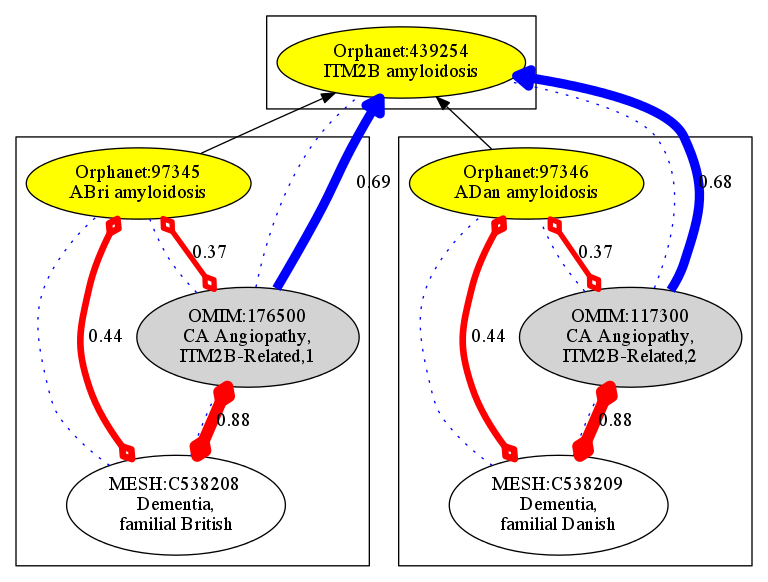
\includegraphics[width=7cm]{amyloidosis}
\caption{Module resolution graph exported by kBOOM; equivalence=red,
  subclass=blue, dashed=supplied mapping. Prior probabilities written
  as edge labels (thick lines are more probable). Enclosing boxes
  denote equivalence cliques, which can be merged to a single class. Inferred edges not shown.}
\label{fig:graph}
\end{figure}
%----------------------------------------

\subsection{Tolerance and detection of mapping errors}

When we assign prior probabilities, we assume a low error rate in
source-provided mappings, and thus for larger modules these are rarely
rejected, even if it leads to an overall more probable structure (due
to the greedy selection procedure). As a pre-processing step step we
take large modules and iteratively test removal of axioms to determine
if the module is broken into semantically distinct submodules, which
can sometimes detect incorrect mappings (e.g. \footnote{https://github.com/DiseaseOntology/HumanDiseaseOntology/issues/134}). We
plan to fold this into the probabilistic approach.


%example of resolution of erroneous mapping
% incorrect mapping of DOID to OMIM:607101 ! Deafness, Autosomal Recessive 30
%3272486 [main] INFO  org.monarchinitiative.owlbag.compute.ProbabilisticGraphCalculator  -   CLIQUE MEMBER:OMIM_609706 Deafness, Autosomal Recessive 53
%3272486 [main] INFO  org.monarchinitiative.owlbag.compute.ProbabilisticGraphCalculator  -   CLIQUE MEMBER:DOID_9261 nasopharynx carcinoma
%3272486 [main] INFO  org.monarchinitiative.owlbag.compute.ProbabilisticGraphCalculator  -   CLIQUE MEMBER:OMIM_601369 Deafness, Autosomal Dominant 9
%3272486 [main] INFO  org.monarchinitiative.owlbag.compute.ProbabilisticGraphCalculator  -   CLIQUE MEMBER:OMIM_602459 Deafness, Autosomal Dominant 15

\subsection{Integration with curation}

One advantage of our approach is that it fits well with both manual
curation and knowledge-driven approaches. The more knowledge provided
by a curator, the better the results; at the same time, the approach
is robust to incomplete information, attempting to estimate the most
likely structure, and always producing a coherent result, if it can be
found.

A curator can provide different kinds of information, and this can be
done iteratively. The most basic information to be provided is a
manually vetted curation. Additional information can be in the form of
prior probabilities for different axiom types; for example, if a
curator strongly believes a mapping denotes equivalence, this can be
provided (and if the curator is highly confident, the axiom can be
removed from the probabilistic set and added directly into the
ontology).

The search procedure uses an OWL reasoner, so other axiom types can be
freely used; e.g the curator can provide defining equivalence axioms
to class expressions. The curator can also provide constraints on
possible models using constructs such as disjointness axioms, or taxon
constraints or some of the other logical constraints developed in
GO\cite{Mungall2014} and Uberon.

\subsection{Comparison with other approaches}

There are a number of probabilistic approaches to ontology mapping,
but most are aimed at generating rather than interpreting mapping. One
exception is the OMEN algorithm\cite{Mitra2005} which is similar to
our approach in that it generates probability distributions for axiom
types based on mappings, and factorizes the joint probability
distribution into a bayesian network. However, the approach has
certain assumptions that are problematic for the disease mapping use
cases, such as the combined ontology containing no cycles. We aim to
do further investigation into a generalized approach that unifies OMEN
and kBOOM.

In order to fully evaluate our method, we plan to compare the disease
merging results with other combined disease resources such as MedGen
and EFO\cite{malone2010modeling}. Additionally, we apply on other
domains such as anatomy and compare to gold standards such as Uberon.

\subsection{Algorithm extensions and other Applications}

Our current implementation was designed for the special case of
translating mappings into simple OWL axioms of either the SubClass or
Equivalence type. For other domains, richer OWL constructs would be
useful (for example, existential restrictions, to represent
relationships to members of classes, e.g. partOf). The general
approach can be applied here, but the main challenge will be the
expansion of the search space, requiring more sophisticated approaches
to prune and explore, e.g. MCMC.



% Do NOT remove this, even if you are not including acknowledgments
%\section{Acknowledgments}

%\section{References}
% The bibtex filename
\bibliographystyle{plain}
\bibliography{kboom-mini}


\end{document}
